\documentclass[11pt]{article}
\usepackage[margin=1 in, letterpaper]{geometry}
\usepackage{fontspec, graphicx, amsmath, amssymb, amsthm, array, physics, enumitem, cancel, multicol, float, bm}
\usepackage[dvipsnames]{xcolor}

\setmainfont{Linux Libertine O}
\setsansfont{Linux Biolinum O}
\setmonofont{Latin Modern Mono}
\setmathrm{Latin Modern Math}
\theoremstyle{definition}
\newtheorem{theo}{\color{Maroon} Theorem}[section] 
\newtheorem{defin}[theo]{\color{Maroon} Definition}
\newtheorem{example}[theo]{\color{Maroon} Example}
\newtheorem{prob}[theo]{\color{Maroon} Problem}
% \newtheorem{example}[section]{\color{Maroon} Example}
\usepackage{lscape}
\theoremstyle{remark}
\newtheorem*{soln}{\color{Maroon} Solution}
\usepackage{latexsym, marvosym}

\newcommand{\convas}{\xrightarrow{\text{a.s.}}}
\newcommand{\convprob}{\xrightarrow{\mathbb{P}}}
\newcommand{\convdist}{\xrightarrow{d}}

\newcommand{\R}{\mathbb{R}}
\newcommand{\Q}{\mathbb{Q}}
\newcommand{\Z}{\mathbb{Z}}
\newcommand{\N}{\mathbb{N}}
\newcommand\independent{\protect\mathpalette{\protect\independenT}{\perp}}
\def\independenT#1#2{\mathrel{\rlap{$#1#2$}\mkern2mu{#1#2}}}

%%%%%%%%%%%%%%%%%%% Statistics %%%%%%%%%%%%%%%%%%%%
\newcommand{\E}[1]{\mathbb{E}\left[ #1 \right]}
\newcommand{\Prob}[1]{\mathbb{P}\left[ #1 \right]}
\newcommand{\cov}[2]{\textnormal{Cov}\left[ #1, #2 \right]}
\renewcommand{\var}[1]{\textnormal{Var}\left[ #1 \right]}
% \renewcommand{\var}{\textnormal{Var}}
% \newcommand{\cov}{\textnormal{Cov}}
\newcommand{\Unif}{\textnormal{Unif}}
\newcommand{\Norm}{\mathcal{N}}
\newcommand{\Bin}{\textnormal{Bin}}
\newcommand{\Beta}{\textnormal{Beta}}
\newcommand{\Bern}{\textnormal{Bern}}
\newcommand{\Geom}{\textnormal{Geom}}
\newcommand{\FS}{\textnormal{FS}}
\newcommand{\Expo}{\textnormal{Expo}}
\newcommand{\DUnif}{\textnormal{DUnif}}
\newcommand{\Pois}{\textnormal{Pois}}
\newcommand{\NBin}{\textnormal{NBin}}
\newcommand{\HGeom}{\textnormal{HGeom}}
\newcommand{\Gam}{\textnormal{Gamma}}
\newcommand{\Mult}{\textrm{Mult}}
\newcommand{\iidsim}{\overset{\text{iid}}{\sim}}

%%%%%%%%%%%%%%%%%%%%%%%%%%%%%%%%%%%%%%%%%%%%%%%%%%%%%%%%%%%%%%%%%%%%
\newcommand{\inserttitle}{Section 10}
\newcommand{\insertauthor}{Max Guo \& Seung Hwan An}
\newcommand{\insertcourse}{STAT 110}
%%%%%%%%%%%%%%%%%%%%%%%%%%%%%%%%%%%%%%%%%%%%%%%%%%%%%%%%%%%%%%%%%%%%

\usepackage{fancyhdr}
\setlength{\headheight}{15pt}
\pagestyle{fancy}
\fancyhf{}
\fancyhead[C]{\thepage}
\fancyhead[L]{\inserttitle}
\fancyhead[R]{\insertauthor}

%%%%%%%%%%%%%%%%%%%%%%%%%%%%%%%%%%%%%%%%%%%%%%%%%%%%%%%%%%%%%%%%%%%%

\begin{document}

{\noindent\Huge\bf  \\[0.1\baselineskip] {\inserttitle }}\\[2\baselineskip]
{{\bf \insertcourse}\\ {\textit{November 15, 2021}}} \hfill {\large \textsc{\insertauthor}}
\smallskip

\section{Conditional Expectation and Variance}
\begin{description}
	\item[Properties of Conditioning on Random Variables]. 

	\begin{enumerate}
		\item $\E{Y|X} = \E{Y}$ if $X \independent Y$
		\item (Taking out what's known). \\
		    $\E{h(X)|X} = h(X)$  \\
			$\E{h(X)W|X} = h(X)\E{W|X}$
		\item (Adam's Law) \\ 
		$\E{\E{Y|X}} = \E{Y}$
		\item (Adam's Law with extra conditioning) \\ $\E{\E{Y|X,Z}|Z}=\E{Y|Z}$
	    \item (Projection) \\
	    $Y - \E{Y | X} $ is uncorrelated with $h(X)$ for any function $h$.
	\end{enumerate}

	\item[Law of Total Expectation] For any set of events that partition the sample space, $A_1, A_2, \dots, A_n$ or just simply $A, A^c$, the following holds:
	\begin{align*}
		\E{Y} &= \E{Y|A}\Pr[A] + \E{Y|A^c}\Pr[A^c] \\
		\E{Y} &= \E{Y|A_1}\Pr[A_1] + \E{Y|A_2}\Pr[A_2] + \dots + \E{Y|A_n}\Pr[A_n]
	\end{align*}
	
	\item[Eve's Law] The interpretation is that the total variance is the sum of ``within-group'' variation ($\E{\var{Y|X}}$) and ``between-group'' variation ($\var{\E{Y|X}}$) $$\var{Y} = \E{\var{Y|X}} + \var{\E{Y|X}}$$
	
\end{description}

\pagebreak

\section{Inequalities}

\begin{description}

    \item[Cauchy Schwarz]
    
    For any two r.v.s $X,Y$ with finite second moment, $$\E{XY} \leq \sqrt{\E{X^2}\E{Y^2}} $$ with the equality achieved iff $X = cY$ almost surely for some constant $c$.
    
    \item[Jensen's]
    
    For any r.v. $X$ and convex function $g$, $$ \E{g(X)} \geq g(\E{X})$$ with equality achieved iff $g(X) = a + b X$ for some constant $a,b$ almost surely. The opposite inequality is true for concave function $f$: $\E{f(X)} \leq f(\E{X})$. 

    \item[Markov]
    
    For any r.v. $X$ and constant $a > 0$, $$ \Pr[ |X| \geq a ] \leq \E{|X|} / a $$ Note that this is an incredibly general statement about bounding the tails of $X$. In particular, it makes no assumption about $X$! 
    
    \item[Chebyschev] If $X$ has finite mean $\mu$ and variance $\sigma^2$, then for any $a > 0$, $$\Pr[\abs{ X - \mu} \geq a] \leq \frac{\sigma^2}{a^2} $$ Chebyschev tells you that a random variable cannot be with high probability very far away from the mean. 
    
    \item[Chernoff]

    For any r.v. $X$ and constants $a, t > 0$, $$\Pr[ X \geq a ] \leq \frac{\E{e^{tX}}}{e^{ta}} $$ It turns out that for many cases, Chernoff bounds give very tight bounds on $X$. In particular, this is true for any $t$, so we can choose $t$ such that the RHS of the inequality is minimized. For instance, if we were to put bounds on $\Pr[|Z| > 3] = 2 \Pr[Z > 3]$ for $Z \sim \Norm(0,1)$, then by Chernoff, this is $\leq 2 e^{-3t} \E{e^{tZ}} = 2 e^{t^2/2-3t}$. In particular the RHS is a function of $t$ that achieves its minimum value when $t=3$. Hence plugging in $t=3$, we get that $\Pr[|Z|>3] \leq 2e^{-9/2}$.  

\end{description}

\pagebreak

\section{Limit Theorems}

\begin{description}

    \item[Law of Large Numbers] \textbf{Strong} LLN states that given iid $X_1, \ldots, X_n$ with finite expectation $\mu$, for $$ \bar{X}_n = \frac{1}{n} \sum_{i=1}^n X_i $$ we have that as $$\Pr[ \bar{X}_n \to \mu ] = 1$$ That is, with probability 1, $\bar{X}_n$ converges to $\mu$. \textbf{Weak} LLN states that for all $\epsilon > 0$, $$\Pr[\abs{X_n - \mu} > \epsilon] \to 0$$ (this is called convergence in probability). Essentially, LLN states that the sample mean converges to true mean with probability 1. 
    
    \begin{center}
        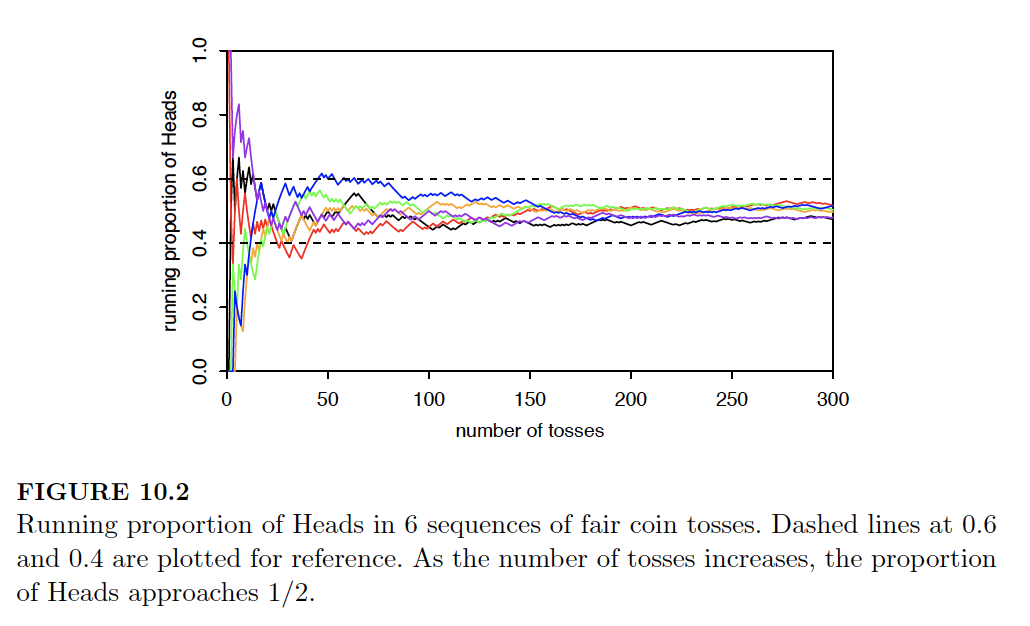
\includegraphics[width=0.8\textwidth]{image/WLLN.png}
    \end{center}
    
    \Biohazard \ For LLN to work, $X_i$ needs to have \textit{finite} expectation (otherwise, what would it converge to?). All distributions we worked with so far had finite expectation, but there are distributions out there that doesn't, like the Cauchy distribution, which is the distribution of $Z_1 / Z_2$ for $Z_1, Z_2 \iidsim \Norm(0,1)$. 
    
    \begin{center}
        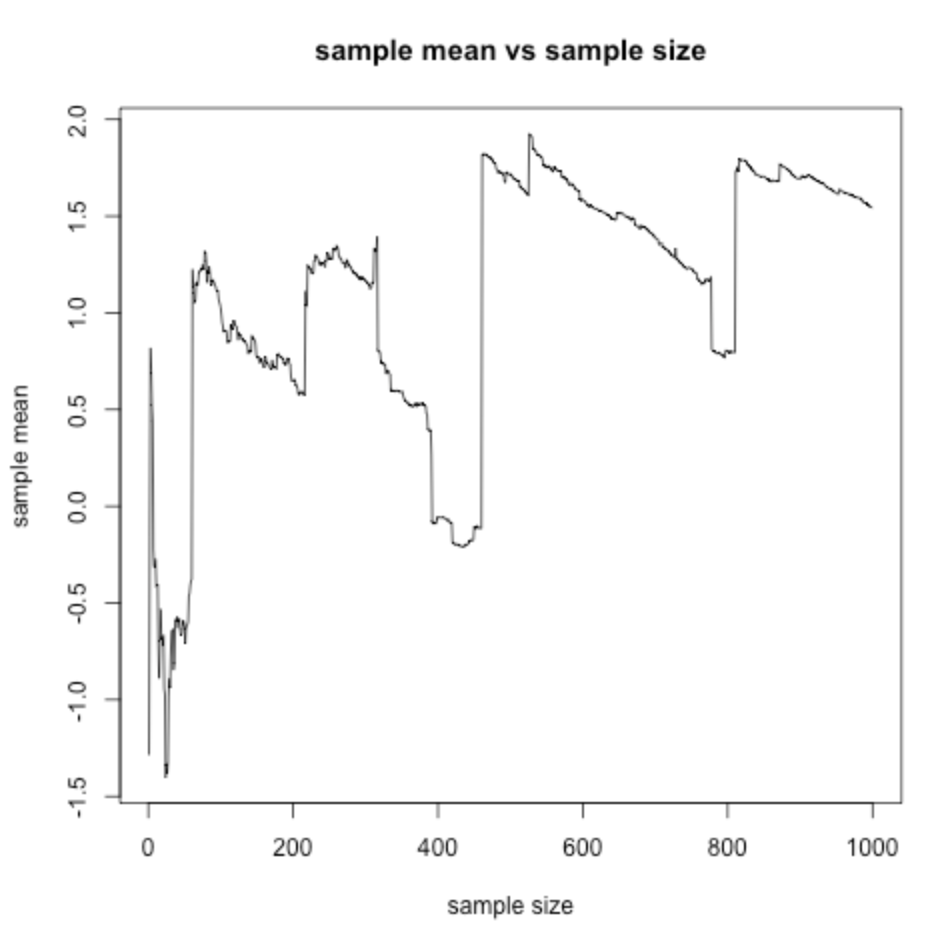
\includegraphics[width=0.5\textwidth]{image/cauchysample.png} \\
        The following is the plot of sample mean of Cauchy distribution versus sample size. \\
        Note that the sample mean does \textit{not} converge to a single value.
    \end{center}

    \item[Central Limit Theorem]

    Central limit theorem tells us the limiting behavior of the sample mean. For $X_i \sim (\mu, \sigma^2)$ (has mean $\mu$ and variance $\sigma^2$), $$ \sqrt{n} \left( \frac{\bar{X}_n - \mu}{\sigma} \right) \to \Norm(0,1) \text{ in distribution}$$

    Note that LLN tells us $\bar{X}_n$ converges (in probability, and thus in distribution) to the true mean. CLT tells you that the distance of sample mean from the true mean, standardized by dividing by $\sigma$, and then \textbf{multiplying} $\sqrt{n}$, we get a standard normal distribution.
    
    Another way to state the CLT is that $\bar{X}_n$ is approximately $\Norm(\mu, \sigma^2/n)$ for sufficiently large $n$. This makes intuitive sense, as more and more sample you get, variance of your sample mean should get smaller and smaller, since you know by LLN that it eventually should converge to $\mu$.
    
    This fact should be surprising! CLT is true for \textit{any} underlying distribution of $X_i$'s, as long as it has finite mean and expectation (no matter the support, symmetricity, etc.). 

    For instance, if you take $X_1, \ldots, X_n \sim \Expo(1)$, and compute $\bar{X}_n$, we will see that $$\frac{\bar{X}_n - 1}{\sqrt{n}} \to \Norm(0,1) \text{ in distribution} $$ even though exponential distribution is extremely skewed, has only positive support, and looks nothing like normal distribution. 

    \Biohazard \ Like the LLN, CLT has the assumption that $X_i$ must have both \textit{finite mean} and \textit{finite variance}.

\end{description}

\pagebreak

\section{Markov Chain}

\begin{description}

    \item[Definition] A discrete state, discrete time \textbf{Markov chain} is a sequence of random variables $X_0, X_1, X_2, \ldots$ such that $X_i \in \mathcal{S}$ where $\mathcal{S} = \{1, 2, \ldots, M\}$ is the \textbf{state space} and satisfies the \textbf{Markov property} that: $$\Pr[X_{n+1} = j | X_n = i, X_{n-1} = i_{n-1}, \ldots, X_0 = i_0 ] = \Pr[ X_{n+1} = j | X_{n} = i ] \equiv \bm{Q}_{ij}$$ That is, the future, \textit{conditioned on the present}, is independent of the past. 
    
    \item[Transition Matrix] \textbf{Transition matrix} $\bm{Q}$ is defined such that $\bm{Q}_{ij}$ is the probability to go from state $i$ to state $j$. Note that transition matrix must be \textbf{stochastic}, in that its rows must sum up to 1 (the probability of transitioning somewhere from state $i$ is 1!): $$ \forall i \in \mathcal{S}, \quad \sum_{j \in \mathcal{S}} \bm{Q}_{ij} = 1 $$ 
    
    \item[Example] Consider a two-state Markov chain with transition matrix $$\bm{Q} = \pmqty{ 0.1 & 0.9 \\ 0.4 & 0.6 } $$ This means that if I am currently at state 1, I stay with probability $0.1$ and move to state 2 with probability $0.9$, and if I am currently at state 2, I stay with probability $0.6$ and move to state 1 with probability $0.4$. 
    
    \item[$n$-step Transition] What is the probability that if I am at state $i$, that I go to state $j$ in two steps? By LOTP, \begin{align*} \Pr[X_{n+2} = j | X_{n} = i] & = \sum_{k \in \mathcal{S}} \Pr[X_{n+2} = j | X_{n} = i , X_{n+1} = k] \Pr[X_{n+1}=k | X_n = i] \\
    & = \sum_{k \in \mathcal{S}} \Pr[X_{n+2} = j | X_{n+1} = k] \Pr[X_{n+1}=k | X_n = i] \\
    & = \sum_{k \in \mathcal{S}}\bm{Q}_{ik}\bm{Q}_{kj} \\ 
    & = \left(\bm{Q}^2\right)_{ij} \end{align*} In general, the $n$-step transition matrix is $\bm{Q}^n$.
    
    \item[Marginal distribution of $X_n$] To get marginal distribution of $X_n$, we need to be given the marginal distribution of $X_0$. Denote $\bm{t} = (t_1, \ldots, t_M)$ to be a vector such that $t_i = \Pr[X_0 = i]$ (vector whose components is just the PMF of $X_0$). Then, by LOTP, $$\Pr[X_n = j] = \sum_{i \in \mathcal{S}} \Pr[X_n = j| X_0 = i] \Pr[X_0 = i] = \sum_{i=1}^m t_i (\bm{Q}^n)_{ij} = (\bm{t} \bm{Q}^n)_j $$
    
    \item[Recurrent and Transient States] We can classify states of $\mathcal{S}$ to be either recurrent or transient. State $i \in \mathcal{S}$ is \textbf{recurrent} if the probability of eventually returning to state $i$ is $1$. Otherwise, the state is \textbf{transient}.
    
    \item[Irreducibility] A Markov chain is \textbf{irreducible} if for all states $i,j \in \mathcal{S}$, there exists $n > 0$ such that $(\bm{Q})^n_{ij} > 0$. That is, it is possible to eventually go from any state to any other state. For an irreducible Markov chain, all of its states are recurrent.
    
    \item[Periodicity] A \textbf{period} of state $i$ is the greatest common divisor of all possible number of steps it takes to return to $i$ starting from state $i$. A state is \textbf{aperiodic} if its state is 1, and the Markov chain is aperiodic if all its states are aperiodic. Markov chain is periodic otherwise.
    
    \item[Stationary Distribution] A stationary distribution $\bm{s} = (s_1, \ldots, s_M)$ of a Markov chain is a probability distribution ($s_i \geq 0$, and $\sum_{i \in \mathcal{S}} s_i = 1$) such that $$ \bm{s} = \bm{s} \bm{Q} $$ That is, it is the eigenvector of the transition matrix with eigenvalue $1$. 
    
    If Markov chain starts out with the stationary distribution, then, it remains at that distribution forever.
    
    \item[Existence of unique stationary distribution] For any irreducible Markov chain, there exists a unique stationary distribution. 
    
    \item[Convergence Theorem] If a Markov chain is irreducible and aperiodic, and has stationary distribution $\bm{s}$, then for \textit{any} starting distribution, the distribution of $X_n$ converges to $\bm{s}$. 
    
    \item[Expected time to Return] If an irreducible Markov chain has stationary distribution $\bm{s}$, and we denote $r_i$ to be the expected time it takes for the chain return to $i$ after starting at state $i$, then $s_i = 1/r_i$.
    
    \item[Reversibility] Let $\bm{Q}$ be the transition matrix of a Markov chain. Suppose there exists a distribution $\bm{s}$ such that $s_i \bm{Q}_{ij} = s_j \bm{Q}_{ji}$ for all states $i,j \in \mathcal{S}$. Then the state is reversible with respect to $\bm{s}$.
    
    Then, $\bm{s}$ is stationary distribution of the chain. (This is an easier way of finding stationary distribution)
    
\end{description}

\pagebreak

\section{Practice Problems}

\begin{prob} \textbf{(Borel's Paradox)}

Suppose that $X_1, X_2 \iidsim \Expo(1)$. Consider $\alpha = \E{X_1 | X_1 = X_2}$.

On one hand, we can calculate $\alpha$ by noting that \begin{align*}
    \E{X_1|X_1=X_2} & = \E{X_1 \Big| \frac{X_1}{X_1+X_2} = \frac{1}{2}} \\
    & = \E{\frac{X_1}{X_1+X_2} \cdot (X_1+X_2) \Big| \frac{X_1}{X_1+X_2} = \frac{1}{2}} \\
    & = \frac{1}{2} \E{ X_1+X_2 \Big| \frac{X_1}{X_1+X_2} = \frac{1}{2}} \\
    & = \frac{1}{2} \E{ X_1+X_2 } = 1
\end{align*} where we use the bank-post office result that $X_1+X_2$ and $X_1/(X_1+X_2)$ is independent.

On the other hand, $|X_1-X_2|=\max(X_1,X_2)-\min(X_1,X_2)$. We know that $\min(X_1,X_2) \sim \Expo(2)$ and is independent of $|X_1-X_2|$ by the memoryless property. Therefore, \begin{align*}
    \E{X_1|X_1=X_2} & = \E{X_1 | |X_1-X_2| = 0} \\
    & = \E{ \min(X_1,X_2) | |X_1-X_2| = 0} \\
    & = \E{ \min(X_1,X_2) } \\
    & = 1/2
\end{align*} giving us a different answer! So what went wrong?

\medskip

\fbox{\parbox{0.9 \textwidth}{The problem is not with our logic in either methods. The problem lies with $\alpha = \E{X_1|X_1=X_2}$ itself. Note that we are conditioning on the event $X_1=X_2$, but this event has probability zero! Note that our definition of conditional probability and expectation breaks when we condition on events with probability zero: if $\Pr[B]=0$, then since $\Pr[A|B] \Pr[B] = \Pr[A]$, $\Pr[A]=0$, and $\Pr[A|B]$ can be \textit{any} value. Hence our conditional expectation is undefined in this case. \\

But wait! Haven't we already used conditional probabilities or expectation even when we are conditioning on probability zero event? For instance, $\E{X_1+X_2|X_1=3} = \E{X_2} + 3 = 4$. Clearly event $X_1=3$ has probability zero? \\

The answer is that in this class, for most instances, this does not become an issue. But this problem is an instructive, pathological example of what can go wrong if we don't think about conditional probability and expectation carefully.}}

\pagebreak

\end{prob}

\begin{prob} \textbf{(Cauchy Schwarz)} Show that for any two r.v.s, $\text{SD}(X+Y) \leq \text{SD}(X)+\text{SD}(Y)$.

\fbox{\parbox{0.9 \textwidth}{This is because $$\text{SD}(X+Y) = \sqrt{ \var{X+Y}} = \sqrt{ \var{X} + \var{Y} + 2 \cov{X}{Y}}$$ and $$\text{SD}(X)+\text{SD}(Y) = \sqrt{ \var{X} + \var{Y} + 2 \sqrt{ \var{X} \var{Y}}} $$ Hence it boils down to comparing $\cov{X}{Y}$ and $\sqrt{ \var{X} \var{Y}}$. We know that the left term is greater by Cauchy Schwarz, since we can take $X,Y$ to be centered (shifting r.v.s do not affect their variance or covariance), so $\cov{X}{Y} = \E{XY}$ and $\var{X} = \E{X^2}$ and $\var{Y} = \E{Y^2}$. Apply Cauchy Schwarz to get the inequality.}}

% \vspace{ 1.5 in }

\end{prob}

\begin{prob} \textbf{(BH. 10.12)} Let $X,Y$ be two nonnegative r.v.s, not necessarily independent. Assume that all expressions below exist (like expectation). Write the most appropriate of $\leq, \geq, =$, or $?$ (meaning no relationship holds in general). 

\begin{enumerate}[label=(\alph*)]
    \item $\Pr[X+Y > 2]$ \_\_ $(\E{X}+\E{Y})/2$
    \item $\Pr[X+Y > 3]$ \_\_ $\Pr[X > 3]$
    \item $\E{\cos(X)}$ \_\_ $\cos(\E{X})$
    \item $\E{X^{1/3}}$ \_\_ $(\E{X})^{1/3}$
    \item $\E{X^{Y}}$ \_\_ $(\E{X})^{\E{Y}}$
    \item $\E{\E{X|Y}+\E{Y|X}}$ \_\_ $\E{X}+\E{Y}$
\end{enumerate}

	\fbox{\parbox{0.9 \textwidth}{
	
	\begin{enumerate}[label=(\alph*)]
	    \item The first inequality is $\leq$ by Markov inequality.
		\item The second inequality is $ \geq $ since $X > 3$ implies $X + Y > 3$. 
		\item The third inequality is $?$ since cosine is convex on certain intervals (like $(\pi/2, 3\pi/2)$]) and concave on others (like $(3\pi/2,5\pi/2)$).
		\item The fourth inequality is $\leq$ since $x^{1/3}$ is a concave function on the positive interval. 
        \item The fifth inequality is $?$, since we can let $Y = 2$, in which case by Jensen is $\geq$ and $Y=1/2$, in which case by Jensen is $\leq$.
        \item The last inequality is $=$ by linearity and Adam' law.
	\end{enumerate} }}

\end{prob}

\pagebreak

\begin{prob} (\textbf{BH. 10.26}) \begin{enumerate}[label=(\alph*)]
    \item Explain why $\Pois(n)$ distribution is approximately normal for large $n$. Specify the parameters of such normal distribution.
    
    \fbox{\parbox{0.9 \textwidth}{Remember that for independent $X_1, \ldots, X_n \iidsim \Pois(1)$, $X = \sum_{i=1}^n X_i \sim \Pois(n)$. Hence by CLT, we know that $X \overset{\cdot}{\sim} \Norm( n \E{X_i}, n \var{X_i} ) = \Norm(n,n)$.}} 
    
    % \vspace{ 2 in }
    
    \item Stirling's formula is an amazingly accurate approximation for factorials: $$ n! \approx \sqrt{2\pi n} \left( \frac{n}{e} \right)^n $$ where in fact the ratio fo the two sides goes to 1 as $n \to \infty$. Use (a) to derive a quick heuristic derivation of Stirling's formula by using a Normal approximation to the probability that a Pois($n$) r.v. is $n$, with the continuity correction: first write $\Pr[N=n] = \Pr[n-1/2 < N < n + 1/2]$ where $N \sim \Pois(n)$. 
    
    \fbox{\parbox{0.9 \textwidth}{By part (a), $$ \Pr[N = n] \approx \Pr[n-1/2 < \sqrt{n} Z + n < n + 1/2] $$ for $ Z \sim \Norm(0,1)$. Hence, the probability is approximately $$ \Pr\left[ - \frac{1}{2\sqrt{n}} < Z < \frac{1}{2\sqrt{n}}  \right] $$ For large $n$, this interval is really small. Hence this probability (using the limit definition of PDF) is PDF of standard normal at zero times the length of the interval, which is $$ \frac{1}{\sqrt{2\pi}} \cdot \frac{1}{\sqrt{n}} $$ But, we can directly compute $$\Pr[N= n] = \frac{n^n e^{-n}}{n!} $$ Setting these two values equal to each other, we get $$ n! \approx \sqrt{2\pi n} \left( \frac{n}{e} \right)^n $$}}
    
\end{enumerate}
\end{prob}

\pagebreak

\begin{prob} (\textbf{Ehrenfest Model})

Suppose that you have a box with $N$ molecules, separated into two halves by a partition with a hole in it. Think of the two partitions as two urns containing balls labeled 1 through $N$. Molecular motion can be modeled by choosing a number between $1$ and $N$ at random and moving the corresponding ball from the urn it is presently in to the other. This is a historically important physical model introduced by Ehrenfest in the early days of statistical mechanics to study thermodynamic equilibrium.  

Let $\{X_0, X_1, \ldots\}$ be a Markov chain keeping track of the number of molecules on one side of the partition, with $X_i \in \{0,1,\ldots,N\}$. 

\begin{enumerate}[label = (\alph*)]
    \item What is the transition matrix $\bm{P}$?
    
    % \vspace{1.5 in} 
    
    \fbox{\parbox{0.9 \textwidth}{Given $X_n$, $X_{n+1}$ can either be $X_n + 1$ or $X_n - 1$. If the ball that is randomly chosen is one of the $X_n$ balls, then it becomes $X_{n}-1$ and if it isn't, then $X_n + 1$. Therefore, $$\bm{P}_{ij} = \Pr[X_{n+1}=j | X_{n} = i] = \begin{cases} i/N & \qif j = i - 1 \\ (N - i)/N & \qif j = i + 1 \end{cases} $$}}

    \item What is the stationary distribution of the chain?
    
    \fbox{\parbox{0.9 \textwidth}{First, denote $p_i = (N-i)/N$ and $q_i = i/N$. Then, since the stationary distribution must satisfy $\bm{s} \bm{P} = \bm{s}$, \begin{align*}
        s_0 & = s_1 q_1 \\
        s_1 & = s_0 p_0 + s_2 q_2 \\
        s_2 & = s_1 p_1 + s_3 q_3 \\
        & \vdots \\
        s_i & s_{i-1} p_{i-1} + s_{i+1} q_{i+1} \\
        & \vdots \\
        s_N & = s_{N-1} p_{N-1}
    \end{align*}
    
    We attempt to represent a generic $s_i$ in terms of $s_0$. To do this, note that \begin{align*}
        s_1 & = \frac{1}{q_1} s_0 \\
        s_2 & = \frac{1}{q_2} \left( s_1 - s_0 p_0 \right) = \frac{1}{q_2 q_1} \left( 1 - q_1 p_0 \right) s_0 = \frac{p_1}{q_2q_1} s_0 \\
        & \vdots
    \end{align*}
    
    We can prove by induction that $$s_i = \frac{p_{i-1} p_{i-2} \ldots p_0}{q_i q_{i-1} \ldots q_1} s_0 = \frac{(N-i+1) \ldots N}{i(i-1) \ldots 1} s_0 = \binom{N}{i} s_0$$ Since $\bm{s}$ is a probability distribution it must sum up to 1, and we know that $s_0 = 2^{-N}$ will normalize the distribution (since this a $\Bin(N,1/2)$ distribution!) Hence, a stationary distribution is $\Bin(N,1/2)$ distribution!}}
    
    \pagebreak
    
    \item For a large $N$ can we approximate the stationary distribution with a normal distribution? If so, with what parameters?
    
    % \vspace{ 1.5 in } 
    
    \fbox{\parbox{0.9 \textwidth}{Remember the story of a binomial - that it is the sum of $N$ iid Bernoulli $\Bern(1/2)$. Hence, by CLT, we can approximate this distribution with $\Norm(N/2,N/4)$. 
    
    For a reasonable $N$ for number of gas molecules in a small pocket of air is $N \approx 10^{24}$. This means that the number of molecules on the left side of the partition is about $0.5 \times 10^{24}$ with \textit{standard deviation} of around $0.5 \times 10^{12}$, which is much much smaller than the mean. This tells us that the number of molecules on the left is basically the same as the number of molecules on the right, which is what you would expect intuitively - but the Ehrenfest model showed that this \textit{macroscopic} property of gas molecules resulted from \textit{microscopic} physics of gas molecules.
    
    Perhaps unsurprisingly, many of the earlier works on Markov chain was done by physicists!}}
    
    \item What is the number of steps it takes on average for a partition to become empty given that it was initially empty? (i.e. expected time to return to state $0$ given that it started out at $0$)

    \fbox{\parbox{0.9 \textwidth}{Since this is an irreducible, thus recurrent chain, the expected return time is inverse of the stationary distribution at state 0, which is $2^{-N}$. Hence the expected return time is $2^N$. }}
    
\end{enumerate}

\end{prob}

\pagebreak

\section{Appendix: Fun with Convergence}

In strong LLN, weak LLN, and CLT we saw three different types of convergences:
\begin{enumerate}
    \item \textbf{Almost sure convergence}: $\Pr[ \lim_{n \to \infty} X_n = X] = 1$
    \item \textbf{Convergence in probability}: For all $\epsilon > 0$, $\Pr[ |X_n - X| > \epsilon ] \to 0$.
    \item \textbf{Convergence in distribution}: If $F_n(x)$ is the CDF function of $X_n$, and $F(x)$ is the CDF function of $X$, then $\forall x \in \R$, $\lim_{n \to \infty} F_n(x) \to F(x)$. 
\end{enumerate}

We denote almost sure convergence as $X_n \convas X$, convergence in probability as $X_n \convprob X$, and convergence in distribution as $X_n \convdist X$. Now, does:

\begin{enumerate}[label = (\alph*)]
    \item $X_n \convas X \implies X_n \convprob X$?
    \item $X_n \convprob X \implies X_n \convdist X$?
    \item $X_n \convprob X \implies X_n \convas X$?
    \item $X_n \convdist X \implies X_n \convprob X$?
\end{enumerate}

It turns out that (a) and (b) is true. Convergence a.s. implies in probability, which implies in distribution. However, the converses (c) and (d) turns out to be false. Here is the counter-example.

Counterexample to (c) is the following: take $X_n \sim \Bern(1/n)$. Then, for any $0 < \epsilon < 1$, $$\Pr[|X_n|> \epsilon ] = \frac{1}{n} \to 0 $$ and hence $X_n \convprob 0$. However, $$\Pr[ \lim_{n \to \infty} X_n = 0] \approx \Pr\left[ \text{at certain }N, \text{ for all } n \geq N, X_n = 0 \right] \leq \left(1 - \frac{1}{N}\right)\left(1 - \frac{1}{N+1}\right) \cdots $$ Note that the last term can be written as $$ \frac{N-1}{N} \frac{N}{N+1} \frac{N+1}{N+2} \cdots $$ which becomes $$\frac{N-1}{\text{very large number that diverges}}$$ Hence in any case, this probability is not 1. (This proof is quite informal, since $N$ is not fixed, and is in fact random, but full proof requires more complicated math I don't want to get into here) Hence, $X_n \not\convas X$.

Counterexample to (d) is much more simple. Let $X \sim \Norm(0,1)$ and $Y = -X$. Clearly $Y$ is equal to $X$ in distribution and hence trivially converges to $X$ in distribution. Yet for any $\epsilon > 0$, $$\Pr[ |Y - X| > \epsilon ] $$ certainly does not go to zero since $X - Y$ is distributed $\Norm(0,4)$.

And the fun with convergence does not stop here! Turns out there are many other different types of convergences that probabilists deal with regular frequency, such as convergence in expectation (that $\E{X_n} \to \E{X}$) or uniform convergence. Take STAT 210 to explore this wonderful and terrifying world of convergence!

\end{document}